% Options for packages loaded elsewhere
% Options for packages loaded elsewhere
\PassOptionsToPackage{unicode}{hyperref}
\PassOptionsToPackage{hyphens}{url}
\PassOptionsToPackage{dvipsnames,svgnames,x11names}{xcolor}
%
\documentclass[
  10pt,
  letterpaper,
  DIV=11,
  numbers=noendperiod]{scrartcl}
\usepackage{xcolor}
\usepackage{amsmath,amssymb}
\setcounter{secnumdepth}{-\maxdimen} % remove section numbering
\usepackage{iftex}
\ifPDFTeX
  \usepackage[T1]{fontenc}
  \usepackage[utf8]{inputenc}
  \usepackage{textcomp} % provide euro and other symbols
\else % if luatex or xetex
  \usepackage{unicode-math} % this also loads fontspec
  \defaultfontfeatures{Scale=MatchLowercase}
  \defaultfontfeatures[\rmfamily]{Ligatures=TeX,Scale=1}
\fi
\usepackage{lmodern}
\ifPDFTeX\else
  % xetex/luatex font selection
\fi
% Use upquote if available, for straight quotes in verbatim environments
\IfFileExists{upquote.sty}{\usepackage{upquote}}{}
\IfFileExists{microtype.sty}{% use microtype if available
  \usepackage[]{microtype}
  \UseMicrotypeSet[protrusion]{basicmath} % disable protrusion for tt fonts
}{}
% Make \paragraph and \subparagraph free-standing
\makeatletter
\ifx\paragraph\undefined\else
  \let\oldparagraph\paragraph
  \renewcommand{\paragraph}{
    \@ifstar
      \xxxParagraphStar
      \xxxParagraphNoStar
  }
  \newcommand{\xxxParagraphStar}[1]{\oldparagraph*{#1}\mbox{}}
  \newcommand{\xxxParagraphNoStar}[1]{\oldparagraph{#1}\mbox{}}
\fi
\ifx\subparagraph\undefined\else
  \let\oldsubparagraph\subparagraph
  \renewcommand{\subparagraph}{
    \@ifstar
      \xxxSubParagraphStar
      \xxxSubParagraphNoStar
  }
  \newcommand{\xxxSubParagraphStar}[1]{\oldsubparagraph*{#1}\mbox{}}
  \newcommand{\xxxSubParagraphNoStar}[1]{\oldsubparagraph{#1}\mbox{}}
\fi
\makeatother


\usepackage{longtable,booktabs,array}
\usepackage{calc} % for calculating minipage widths
% Correct order of tables after \paragraph or \subparagraph
\usepackage{etoolbox}
\makeatletter
\patchcmd\longtable{\par}{\if@noskipsec\mbox{}\fi\par}{}{}
\makeatother
% Allow footnotes in longtable head/foot
\IfFileExists{footnotehyper.sty}{\usepackage{footnotehyper}}{\usepackage{footnote}}
\makesavenoteenv{longtable}
\usepackage{graphicx}
\makeatletter
\newsavebox\pandoc@box
\newcommand*\pandocbounded[1]{% scales image to fit in text height/width
  \sbox\pandoc@box{#1}%
  \Gscale@div\@tempa{\textheight}{\dimexpr\ht\pandoc@box+\dp\pandoc@box\relax}%
  \Gscale@div\@tempb{\linewidth}{\wd\pandoc@box}%
  \ifdim\@tempb\p@<\@tempa\p@\let\@tempa\@tempb\fi% select the smaller of both
  \ifdim\@tempa\p@<\p@\scalebox{\@tempa}{\usebox\pandoc@box}%
  \else\usebox{\pandoc@box}%
  \fi%
}
% Set default figure placement to htbp
\def\fps@figure{htbp}
\makeatother


% definitions for citeproc citations
\NewDocumentCommand\citeproctext{}{}
\NewDocumentCommand\citeproc{mm}{%
  \begingroup\def\citeproctext{#2}\cite{#1}\endgroup}
\makeatletter
 % allow citations to break across lines
 \let\@cite@ofmt\@firstofone
 % avoid brackets around text for \cite:
 \def\@biblabel#1{}
 \def\@cite#1#2{{#1\if@tempswa , #2\fi}}
\makeatother
\newlength{\cslhangindent}
\setlength{\cslhangindent}{1.5em}
\newlength{\csllabelwidth}
\setlength{\csllabelwidth}{3em}
\newenvironment{CSLReferences}[2] % #1 hanging-indent, #2 entry-spacing
 {\begin{list}{}{%
  \setlength{\itemindent}{0pt}
  \setlength{\leftmargin}{0pt}
  \setlength{\parsep}{0pt}
  % turn on hanging indent if param 1 is 1
  \ifodd #1
   \setlength{\leftmargin}{\cslhangindent}
   \setlength{\itemindent}{-1\cslhangindent}
  \fi
  % set entry spacing
  \setlength{\itemsep}{#2\baselineskip}}}
 {\end{list}}
\usepackage{calc}
\newcommand{\CSLBlock}[1]{\hfill\break\parbox[t]{\linewidth}{\strut\ignorespaces#1\strut}}
\newcommand{\CSLLeftMargin}[1]{\parbox[t]{\csllabelwidth}{\strut#1\strut}}
\newcommand{\CSLRightInline}[1]{\parbox[t]{\linewidth - \csllabelwidth}{\strut#1\strut}}
\newcommand{\CSLIndent}[1]{\hspace{\cslhangindent}#1}



\setlength{\emergencystretch}{3em} % prevent overfull lines

\providecommand{\tightlist}{%
  \setlength{\itemsep}{0pt}\setlength{\parskip}{0pt}}



 


\usepackage{caption}
\captionsetup{font=small, labelfont=bf}
\setlength{\parindent}{0pt}
\setlength{\parskip}{1.25ex}
\KOMAoption{captions}{tableheading}
\makeatletter
\@ifpackageloaded{caption}{}{\usepackage{caption}}
\AtBeginDocument{%
\ifdefined\contentsname
  \renewcommand*\contentsname{Table of contents}
\else
  \newcommand\contentsname{Table of contents}
\fi
\ifdefined\listfigurename
  \renewcommand*\listfigurename{List of Figures}
\else
  \newcommand\listfigurename{List of Figures}
\fi
\ifdefined\listtablename
  \renewcommand*\listtablename{List of Tables}
\else
  \newcommand\listtablename{List of Tables}
\fi
\ifdefined\figurename
  \renewcommand*\figurename{Figure}
\else
  \newcommand\figurename{Figure}
\fi
\ifdefined\tablename
  \renewcommand*\tablename{Table}
\else
  \newcommand\tablename{Table}
\fi
}
\@ifpackageloaded{float}{}{\usepackage{float}}
\floatstyle{ruled}
\@ifundefined{c@chapter}{\newfloat{codelisting}{h}{lop}}{\newfloat{codelisting}{h}{lop}[chapter]}
\floatname{codelisting}{Listing}
\newcommand*\listoflistings{\listof{codelisting}{List of Listings}}
\makeatother
\makeatletter
\makeatother
\makeatletter
\@ifpackageloaded{caption}{}{\usepackage{caption}}
\@ifpackageloaded{subcaption}{}{\usepackage{subcaption}}
\makeatother
\usepackage{bookmark}
\IfFileExists{xurl.sty}{\usepackage{xurl}}{} % add URL line breaks if available
\urlstyle{same}
\hypersetup{
  pdftitle={Image statistic encoding between regions of the visual cortex},
  pdfauthor={Al Xin. Advised by Rob Kass and Jenelle Feather.},
  colorlinks=true,
  linkcolor={blue},
  filecolor={Maroon},
  citecolor={Blue},
  urlcolor={Blue},
  pdfcreator={LaTeX via pandoc}}


\title{Image statistic encoding between regions of the visual cortex}
\author{\small Al Xin. Advised by Rob Kass and Jenelle Feather.}
\date{Sep 24, 2026}
\begin{document}
\maketitle


\pagebreak

\subsection{Introduction}\label{introduction}

Image recognition occurs through the cumulative transformation and
transfer of visual information through successive regions of the brain.
Image processing starts in the primary visual cortex (V1), which
contains neurons that selectively respond to simple image features like
oriented edges. As image information passes through subsequent regions,
such as V2, V4, and IT, each stage contains neurons selective for
progressively higher-level visual features. For instance, the inferior
temporal gyrus (IT), a later visual region, contains neurons that
selectively respond to complex object categories, like hands or flowers
{[}\citeproc{ref-desimone_stimulus-selective_1984}{1}{]}.

While neurons in V1 can be effectively characterized by a few parameters
(namely, the location and direction of an edge), the features relevant
to other regions remain ill-defined. One approach to characterize the
relevant visual features for each layer is through recording neural
responses to visual texture stimuli. Visual textures are approximately
homogeneous images with repeated elements, e.g., images of sand, tree
bark, granite, or honeycomb (Figure~\ref{fig-textures}). Texture
families can be parameterized by a set of image statistics, where image
statistics are \(N\)th-order empirical densities of pixels
{[}\citeproc{ref-portilla_parametric_2000}{2}{]}. Texture images in the
same family can be visually distinct while sharing the same overall
image statistics. Thus, the separability of neural responses to distinct
images from different families compared to distinct images within the
same family provides evidence for how visual information is summarized
in visual areas.

\begin{figure}

\centering{

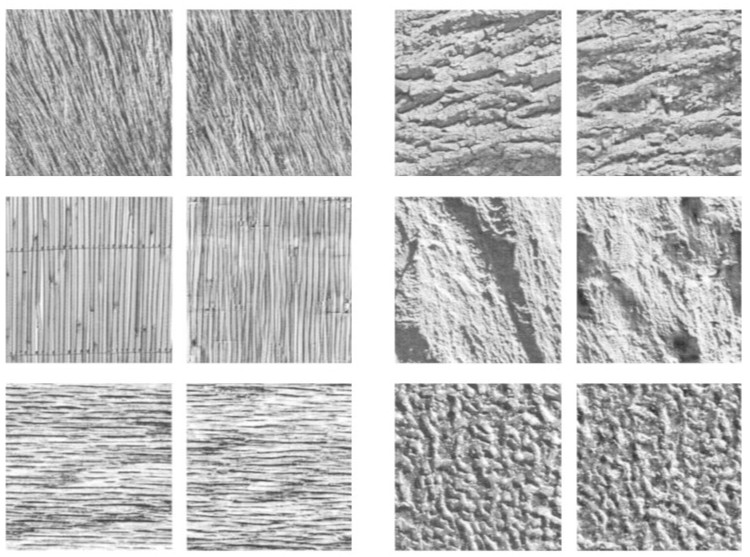
\includegraphics[width=0.5\linewidth,height=\textheight,keepaspectratio]{../img/portilla_simoncelli2000-textures.jpg}

}

\caption{\label{fig-textures}Example naturalistic textures, adapted from
Figure 15 in Portilla and Simoncelli (2000).}

\end{figure}%

Experiments with texture stimuli generally find that higher visual
regions tend to be more selective for higher \(N\)th-order image
statistics. Previously, Ziemba et al.~(2016) found better within-family
separation of neural responses in V1 and better between-family
separation in V2 {[}\citeproc{ref-ziemba_selectivity_2016}{3}{]}.
Relatedly, Okazawa et al.~(2015, 2017) compared the selectivity of V2
and V4 neurons for image statistics in texture stimuli and found V4
neurons tended to be selective for higher order statistics
{[}\citeproc{ref-okazawa_image_2015}{4},\citeproc{ref-okazawa_gradual_2017}{5}{]}.
Other analyses of between-region texture responses found that texture
stimuli with matched higher order image statistics produced higher
firing of V2 and V4 neurons compared to stimuli lacking higher order
image statistics
{[}\citeproc{ref-freeman_functional_2013}{6}--\citeproc{ref-lee_emergence_2025}{8}{]}.
However, existing analyses tend to lack results for the entire visual
processing stream, with few experimenters recording textures responses
in IT. Higher level areas tend to produce sparse responses, so typical
approaches in the literature, such as size-matched population analyses
or single-site neuron metrics, may not produce reliable comparisons
between IT and earlier visual areas.

\pagebreak

\subsection{References}\label{references}

\phantomsection\label{refs}
\begin{CSLReferences}{0}{1}
\bibitem[\citeproctext]{ref-desimone_stimulus-selective_1984}
\CSLLeftMargin{1. }%
\CSLRightInline{R. Desimone, T. D. Albright, C. G. Gross, C. Bruce.
Stimulus-selective properties of inferior temporal neurons in the
macaque. J Neurosci. 1984 Aug 1;4(8):2051--62.
doi:\href{https://doi.org/10.1523/JNEUROSCI.04-08-02051.1984}{10.1523/JNEUROSCI.04-08-02051.1984}}

\bibitem[\citeproctext]{ref-portilla_parametric_2000}
\CSLLeftMargin{2. }%
\CSLRightInline{Javier Portilla, Eero P. Simoncelli. A parametric
texture model based on joint statistics of complex wavelet coefficients.
International Journal of Computer Vision. 2000 Oct 1;40(1):49--70.
doi:\href{https://doi.org/10.1023/A:1026553619983}{10.1023/A:1026553619983}}

\bibitem[\citeproctext]{ref-ziemba_selectivity_2016}
\CSLLeftMargin{3. }%
\CSLRightInline{Corey M. Ziemba, Jeremy Freeman, J. Anthony Movshon,
Eero P. Simoncelli. Selectivity and tolerance for visual texture in
macaque V2. Proc Natl Acad Sci USA. 2016 May 31;113(22).
doi:\href{https://doi.org/10.1073/pnas.1510847113}{10.1073/pnas.1510847113}}

\bibitem[\citeproctext]{ref-okazawa_image_2015}
\CSLLeftMargin{4. }%
\CSLRightInline{Gouki Okazawa, Satohiro Tajima, Hidehiko Komatsu. Image
statistics underlying natural texture selectivity of neurons in macaque
V4. Proceedings of the National Academy of Sciences. 2015 Jan
27;112(4):E351--60.
doi:\href{https://doi.org/10.1073/pnas.1415146112}{10.1073/pnas.1415146112}}

\bibitem[\citeproctext]{ref-okazawa_gradual_2017}
\CSLLeftMargin{5. }%
\CSLRightInline{Gouki Okazawa, Satohiro Tajima, Hidehiko Komatsu.
Gradual development of visual texture-selective properties between
macaque areas V2 and V4. Cereb Cortex. 2017 Oct 1;27(10):4867--80.
doi:\href{https://doi.org/10.1093/cercor/bhw282}{10.1093/cercor/bhw282}}

\bibitem[\citeproctext]{ref-freeman_functional_2013}
\CSLLeftMargin{6. }%
\CSLRightInline{Jeremy Freeman, Corey M. Ziemba, David J. Heeger, Eero
P. Simoncelli, J. Anthony Movshon. A functional and perceptual signature
of the second visual area in primates. Nat Neurosci. 2013
Jul;16(7):974--81.
doi:\href{https://doi.org/10.1038/nn.3402}{10.1038/nn.3402}}

\bibitem[\citeproctext]{ref-lee_developmentally_2024}
\CSLLeftMargin{7. }%
\CSLRightInline{Gerick M. Lee, C. L. Rodríguez Deliz, Brittany N.
Bushnell, Najib J. Majaj, J. Anthony Movshon, Lynne Kiorpes.
Developmentally stable representations of naturalistic image structure
in macaque visual cortex. Cell Reports. 2024 Aug 27;43(8).
doi:\href{https://doi.org/10.1016/j.celrep.2024.114534}{10.1016/j.celrep.2024.114534}}

\bibitem[\citeproctext]{ref-lee_emergence_2025}
\CSLLeftMargin{8. }%
\CSLRightInline{Gerick M. Lee, Najib J. Majaj, C. L. Rodríguez Deliz,
Lynne Kiorpes, J. Anthony Movshon. Emergence of a contrast-invariant
representation of naturalistic texture in macaque visual cortex.
Proceedings of the National Academy of Sciences. 2025 Dec
2;122(48):e2501437122.
doi:\href{https://doi.org/10.1073/pnas.2501437122}{10.1073/pnas.2501437122}}

\end{CSLReferences}




\end{document}
